\section{Sensemaking}
Sensemaking is described as the process by which people give meaning to experience. It has been studied in different contexts such as information science~\cite{Dervin1983}, human-computer interaction~\cite{Russell1993}, and organizational studies~\cite{Weick1995}. In this section, we review two sensemaking models that complement each other and have been highly accepted in the visualization community.

\subsection{Pirolli and Card's Model}
\label{sub:rv-pcm}
Pirolli and Card~\cite{Pirolli2005} describe sensemaking as a iterative process that gradually transforms raw data into rational knowledge. The process includes two sets of activities: one that cycles around finding relevant information, and another that cycles around making sense of the information, with plenty of interaction between them. They map to the \emph{foraging loop} and the \emph{sensemaking loop} respectively, as shown in Figure~\ref{fig:pirolli-card-model}. The sensemaking process can progress upward (from data to knowledge) or downward (from knowledge to data). The steps in the \emph{bottom-up} process are summarized as follows.

\begin{figure}[!htb]
	\centering
	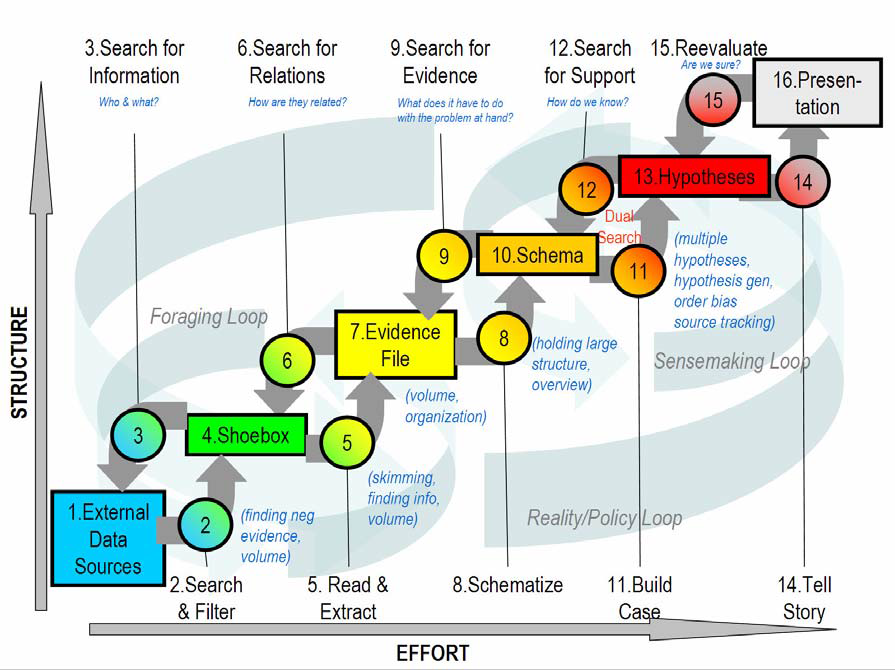
\includegraphics[width=\columnwidth]{pirolli-card-model}
	\caption{A notional model of sensemaking. The sub-processes (numbered circles) and their data input/output (numbered rectangles) are arranged in a two-dimensional space, in which the horizontal axis represents the degree of effort from users, and the vertical axis represents the degree of structure in information representation. \is{\cite{Pirolli2005}}.}
	\label{fig:pirolli-card-model}
\end{figure}

\begin{itemize}
	\item \emph{Search and filter}. External data sources, such as classified databases or the web, are searched and filtered to retrieve relevant documents to the task.
	\item \emph{Read and extract}. These documents are examined to extract pieces of information that may be used as evidence later.
	\item \emph{Schematize}.  The collected information is organized in a way that aids the analysis. This may be executed in user mind, using paper and pen, or with a complex computer-based system.
	\item \emph{Build case}. Multiple hypotheses are generated; evidence are marshaled to support or disconfirm them.
	\item \emph{Tell story}. Discovered cases are presented to some audience.
\end{itemize}

In this model, \emph{schematization} plays an important role in converting raw evidence to rational explanations, bridging the foraging and sensemaking loops. A study by Kang, Görg and John Stasko~\cite{Kang2011} agrees with this observation. In their study, all the participants who performed the sensemaking task well spent considerable time and effort in organizing their collected information. Their organizational schemes were flexible: a \emph{timeline} of related events, a \emph{map} connecting locations that a person has been to, and a \emph{diagram} showing relationships among suspicious targets.

\subsection{Data--Frame Model}
\label{sub:rv-dfm}
Klein et al.~\cite{Klein2003} propose a sensemaking model that centers around \emph{data} and \emph{frame}. Data is the information that a person receives or searches for, and frame is the mental structure that organizes and explains the relationship of data. For instance, a frame can be a \emph{story}, explaining the chronology of events and the causal relationships between
them; or a \emph{map}, showing where the events take place and the routes between them. Sensemaking is considered as a deliberate effort to understand an event, starting when a person realizes a gap of their current understanding of that event. Klein and his associates describe seven activities involved in sensemaking and are summarized in Figure~\ref{fig:data-frame-model}.

\begin{figure}[!htb]
	\centering
	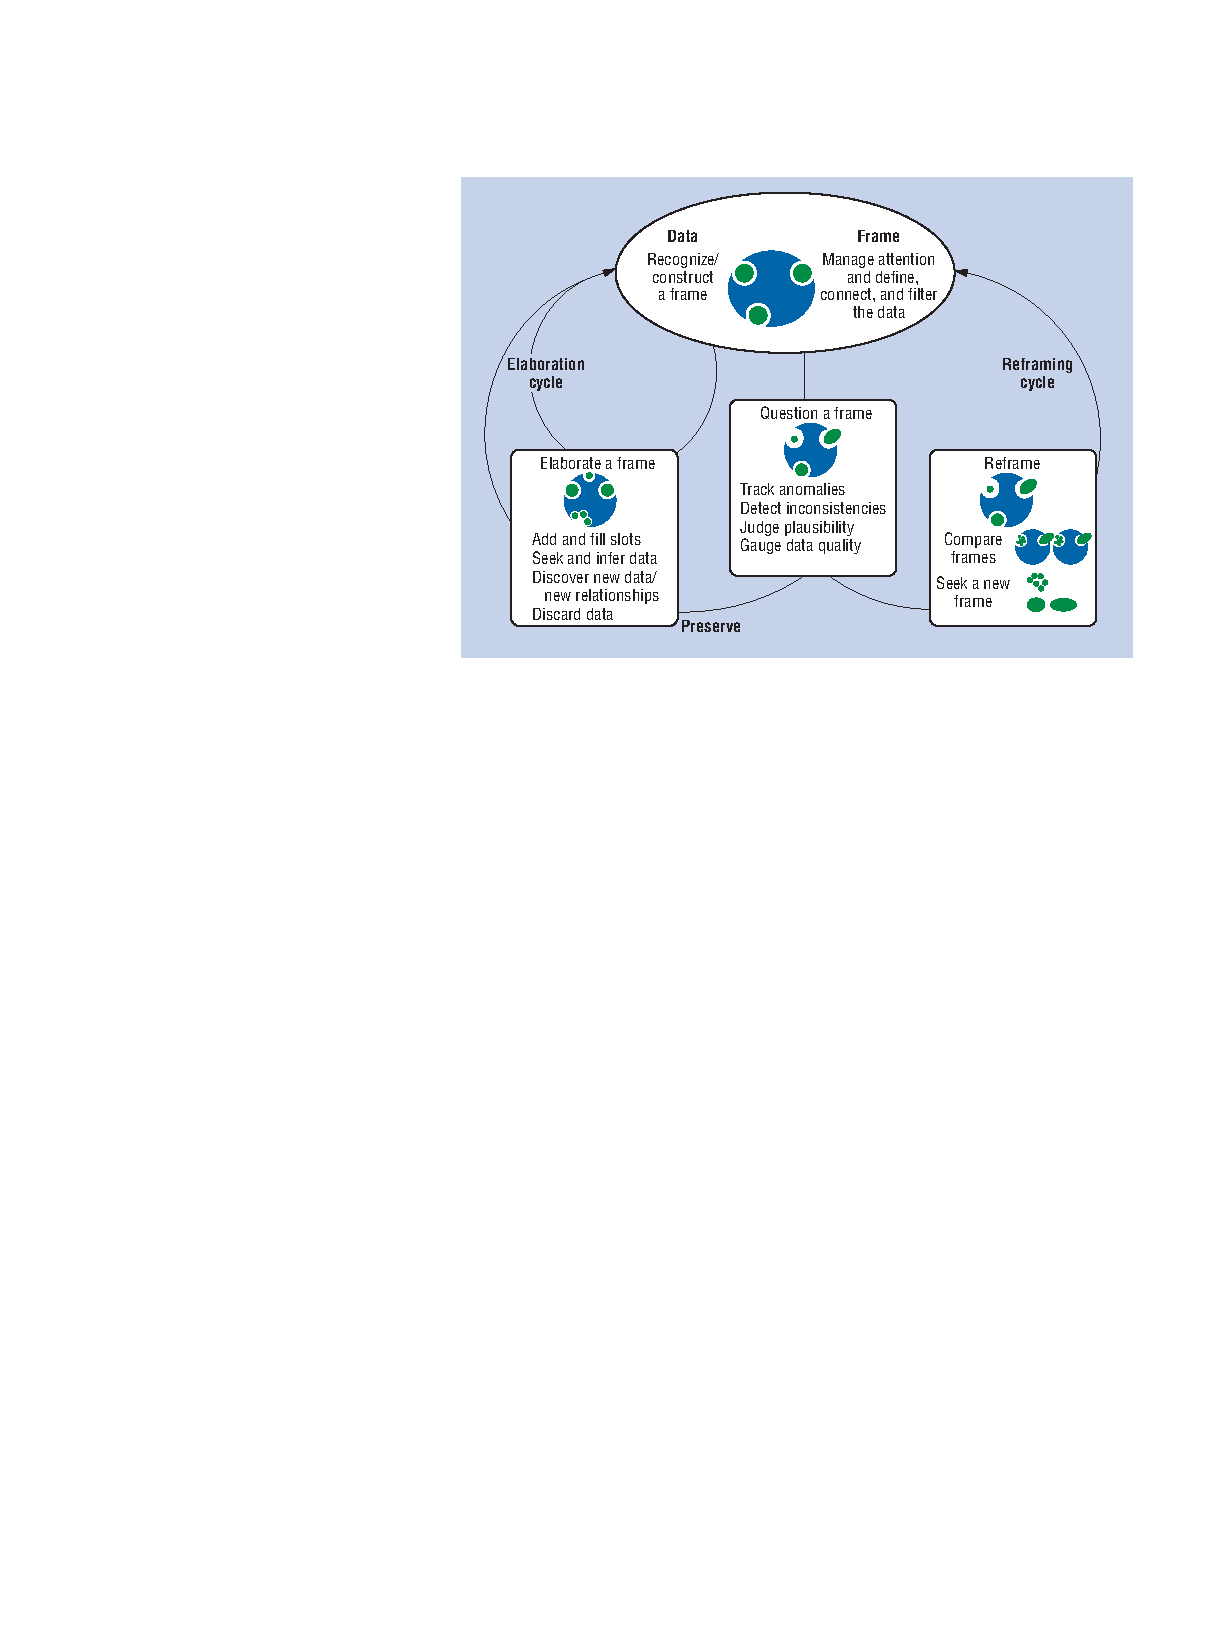
\includegraphics[width=\columnwidth]{data-frame-model}
	\caption{The data--frame model of sensemaking. It describes a set of interconnected sensemaking activities centering around data and frame -- the explanatory structure of data. \is{\cite{Klein2003}}.}
	\label{fig:data-frame-model}
\end{figure}

\begin{itemize}
	\item \emph{Connect data and a frame}. A person recognizes relevant pieces of data and constructs an initial frame to explain them. The frame then helps the person to filter and search for new data.
	\item \emph{Elaborate the frame}. As more is learned about the situation, the frame becomes more elaborate with new data and new relationships. 
	\item \emph{Question the frame}. It happens when a person encounters data that is inconsistent with the existing frame. At this point, the person may be unsure that the frame is incorrect, or the inconsistent data is inaccurate.
	\item \emph{Preserve the frame}. A person may consider the severity of the inconsistent data, justify why it mismatches the frame, and ignore it.
	\item \emph{Compare multiple frames}. Depending on experience, a person may think of alternative frames explaining the same set of data. These frames need to be compared to select the most likely one.
	\item \emph{Reframe}. When encountering inconsistent and contrary data, the person may need to find a replacement that can explain all data. Considering discarded data and/or reinterpreting data could facilitate this activity.
	\item \emph{Seek a new frame}. A person may deliberately search for a new frame when encountering plenty of conflicted data. One or two key data elements may serve as \emph{anchors} to help the person to elicit another frame.
\end{itemize}

The Pirolli and Card's model describes a step-by-step process of sensemaking, in which the analyst collects relevant data and eventually transposes it into rational answers. However, the various sensemaking activities in the Data--Frame model may explain the strategies used by the analyst more comprehensively.